\chapter{Relevant Concepts}
\label{ch:relevant-concepts}

This Section summarizes the relevant concepts which build the foundation of this Thesis.
These include the Semantic Web with annotated and, therefore, machine-readable pages.
We use the data given in those annotations to create a training data set and a foundation for
the product taxonomy matching gold standard.
In the second part of this Chapter, we explain ontologies and taxonomies and how they can be matched.

\section{Semantic Web}
\label{sec:semantic-web}

\subsection{Inception of the Semantic Web}
\label{subsec:semantic-web-concepts}

At the beginning of this century, webpages were optimized for human readers.
They contained a lot of text and some images.
This unstructured information makes it hard for machines to understand the results and to act on them.
Berners-Lee et al.\@~\cite{berners2001semantic} propose the Semantic Web, an extension to the current web,
that is using annotations that make human-readable information accessible to machines.
They propose to use the eXtensible Markup Language (XML) and the Resource Description Framework (RDF) to allow
content-creators to make any part of their page machine-readable or to link it to any other content on the internet.
This approach is very expressive and flexible, but has the limitation that the content consumer must know
what the annotations are about and what they mean.

Berners-Lee et al.\@ propose the RDF syntax based on Unique Resource Identifier (URI) that can be used as primary
keys and combined with predicates.
Assuming there is a database of persons (pe:) and a database of papers (pa:) in which a person can be an author of a paper (authorOf),
we can state that "pe:Berners-Lee authorOf pa:The-Semantic-Web".

Usually, URIs point to web pages, e.g., \url{https://en.wikipedia.org/wiki/Tim\_Berners-Lee}.

\subsection{Realization of the Semantic Web}
\label{subsec:semantic-web-realization}

This Subsection covers how the Semantic Web is implemented today.
We focus on formats to annotate pages and shared vocabularies to compare the contents of different websites.

There are two options to add machine-readable content to a webpage.
The content creator could either annotate the HyperText Markup Language (HTML) elements directly and keep the annotations close to
the human-readable content or add a central property that includes all structured information about the
current page.
The following example from \url{target.com} illustrates the usage of a central object that describes the
current webpage.
The script-tag is placed somewhere inside of the HTML-body and contains all properties that are available
for the given product, like the name, brand, and image.
The type "application/ld+json" indicates that this is a JavaScript Object Notation (JSON) document containing linked data.
\begin{verbatim}
<script class type="application/ld+json">
    {
        "@context": "http://schema.org",
        "@type": "Product",
        "name": "Samsung 50\" Smart 4K UHD",
        "brand": "Samsung",
        "image": "<image-url>",
        "sku": "53832607"
    }
</script>
\end{verbatim}
In the second example, we translated the above ld+json\footnote{\url{https://json-ld.org}. Accessed: 01.05.2020} into microdata annotations.
The HTML snippet could then look like this:
\begin{verbatim}
<div itemtype="http://schema.org/Review">
    <span itemprop="name">Samsung 50\" Smart 4K UHD</span>
    <meta itemprop="brand" content="Samsung" />
    <img itemprop="image" src="<image-url>" />
    <meta itemprop="sku" content="53832607" />
</div>
\end{verbatim}
This would show the product name and the product image, while the other two tags would be hidden from the user.
Nevertheless, the annotation is still closer to human-readable content and, since this content is reused during the
annotation, there can not exist any discrepancies between the machine-readable content and the human-readable content.

One can imagine that both implementations provide a great deal of flexibility and can lead to data silos if there
is no agreement between different pages to use a shared vocabulary.

That is where vocabularies like schema.org or the opengraphprotocol.org come into play.
They provide a shared vocabulary that can be used across webpages to indicate the same meaning.
The examples above already visualized that there are multiple ways to annotate the HTML file.
In the following example, we will compare the machine-readable side with the human-readable one.
\begin{figure}[!htbp]
    \centering
    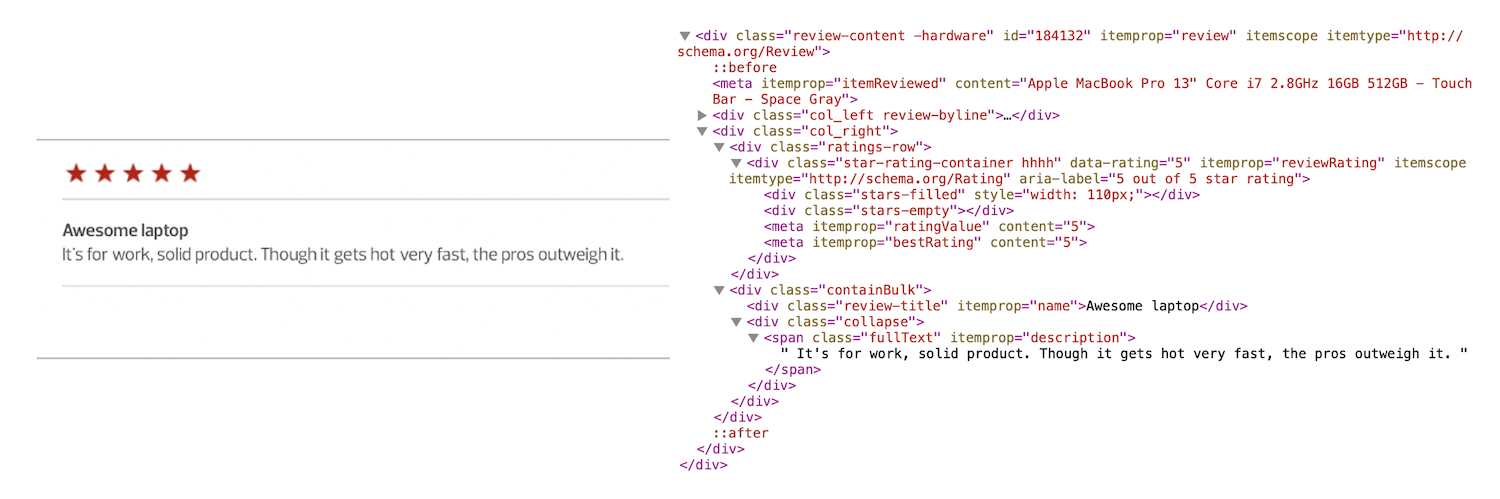
\includegraphics[width=13cm]{images/schema_org_review.png}
    \caption[schema.org/Review Example]{schema.org Review example\protect\footnotemark.
        On the left hand side is the human-readable webpage and on the right hand side is the annotated HTML code.
    }
    \label{fig:schema_org_review}
\end{figure}
\footnotetext{Review source: \url{https://www.cdw.com/product/apple-macbook-pro-13-core-i7-2.8ghz-16gb-512gb-touch-bar-space-gray/5578874}. Accessed: 01.05.2020}
Figure~\ref{fig:schema_org_review} shows an annotated HTML snippet with schema.org annotations
and the corresponding webpage.
The surrounding div-tag declares via the itemtype property that it contains a schema.org/Review.
The definition of a review contains properties like 'itemReviewed' and 'reviewRating'.
In some of the enclosed elements we see the itemprop field, which also maps to the properties specified in the
schema.org/Review.

Now, a computer can parse the same code that is presented to a human and can infer that the itemReviewed
got a reviewRating of 5 stars.
Search engines like Google and DuckDuckGo either use those annotations to enhance the expressiveness of their
results or to immediately respond to questions instead of forwarding the customer to another webpage~\cite{vandic2012faceted}.

\subsection{Working with the Semantic Web}
\label{subsec:semantic-web-working}

The Semantic Web offers an immense potential for data analysis and knowledge generation.
However, due to the distributed setup of the internet, there exists no single source to access all data.
The Billion Triple Challenge~\cite{herrera2019btc} is an attempt at a unified access point, but still contains
only a subset of all available data on the web.
While Herrera et al.\@~\cite{herrera2019btc} provide only raw triples, the WDC
project~\cite{meusel2014webdatacommons}, too, provides triples, but also schema.org class-specific
subsets\footnote{\url{http://www.webdatacommons.org/structureddata/2019-12/stats/schema_org_subsets.html}. Accessed: 01.05.2020}.
This enables researchers to focus on specific data, like Hotels or Product Reviews, without the overhead
of managing all other data.
The WDC project is based on Common Crawl\footnote{\url{http://commoncrawl.org}. Accessed: 01.05.2020} data, a pre-crawled
collection of HTML pages.
The advantage of the Common Crawl dataset is that a researcher does not have to access millions of web pages himself,
but can download the HTML context of those pages from a single source.

In the case that none of the above datasets is sufficient, it is also possible to gather the data directly from the web.
Using frameworks like scrapy\footnote{\url{https://scrapy.org}. Accessed: 01.05.2020} and LDSpider~\cite{isele2010ldspider},
one can retrieve data from a specific set of webpages or get a broad overview of the web.
LDSpider is also used internally for the Billion Triple Challenge.

In this Section, we have seen how semantic annotations make web pages machine-readable and how
shared vocabularies make them also machine-understandable.
The Semantic Web provides infinite opportunities for data-based projects.

\section{Ontologies and Taxonomies}
\label{sec:onto-taxo}

In this Section, we will introduce the concepts of ontologies and, their special case, taxonomies.

In general, ontologies "can be viewed as  a set of  assertions that are meant to model a
particular domain.
Usually, they define a vocabulary used by a particular application"~\cite[p. 25]{euzenat2007ontology}.
A more intuitive way to describe them would be that an ontology is a format or description
that can be used to describe a collection, e.g., database schemata.
Ontologies can range from very informal and expressive, like directories, to a very strict and
formal language, like XML schemas or entity-relation schemas for databases.

According to Euzenat and Shvaiko~\cite[p. 34]{euzenat2007ontology}, ontologies usually consist of the
following entities:
\begin{itemize}
    \item "\textbf{Classes} or concepts are the main entities of an ontology.
          These are interpreted as a set of individuals in the domain. [\ldots]
    \item \textbf{Individuals} or objects or instances are interpreted as a particular individual of a domain. [\ldots]
    \item \textbf{Relations} are the ideal notion of a relation independently to what it applies.
          Relations are interpreted as a subset of the product of the domain. [\ldots]
    \item \textbf{Data types} are particular parts of the domain that specify values.
          Contrary to individuals, values do not have identities. [\ldots]
    \item \textbf{Data values} are simple values. [\ldots]"
\end{itemize}

In this Thesis, we will focus on very informal ontologies, namely taxonomies or directories:
"A taxonomy is a partially ordered set of taxons (classes) in which one taxon is greater than
another only if what the former denotes includes what is denoted by the latter.
Directories or classifications are taxonomies that are used by companies for presenting goods on sale,
by libraries for storing books, or by individuals to classify files on a personal computer"~\cite[p. 27]{euzenat2007ontology}.

Let us look at two examples that are illustrative for the cases above.
The first one is a directory structure on a computer.
Below, we show the layout of our University directory.
The root folder, UniMA, contains all directories listed beneath, e.g., Master Thesis and Organizational.
Those, in turn, contain other directories, which may contain more files.
\begin{verbatim}
> tree -L 2 .
UniMA
|- Master\ Thesis
|   |- Application
|   |- Code
|   |- Data
|   |- Literature
|   |- Thesis
|-  Organizational
    |- FSS18
    |- FSS19
    |- HWS17-18
    |- HWS18-19
    |- HWS19-20
    |- Module\ Catalog\ 17.pdf
    |- Module\ Catalog\ 18.pdf
\end{verbatim}
Inside each directory, there is a clear hierarchy, i.e., it is partially ordered, but we can not infer
any relationships across folders.
For example, we can not say how FSS18 relates to Literature.

Another typical example are online shop taxonomies.
\begin{figure}[!htbp]
    \centering
    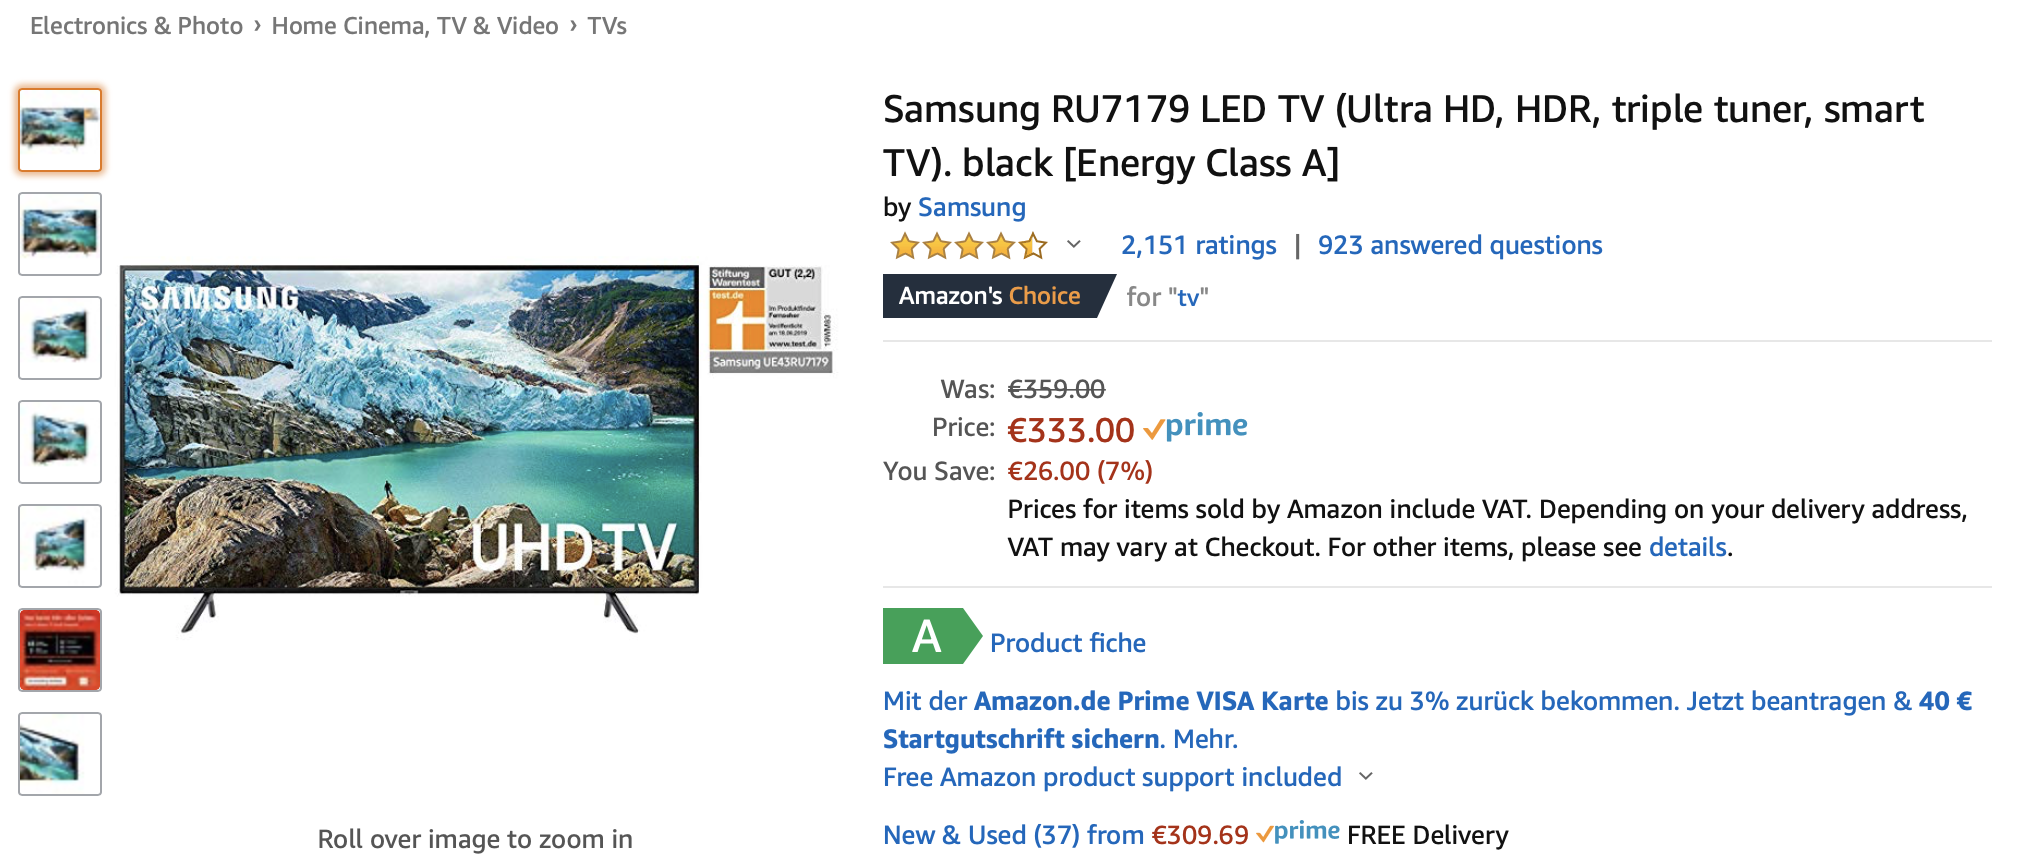
\includegraphics[width=13cm]{images/taxonomy_amazon.png}
    \caption[Amazon Product Screenshot]{Amazon Product Screenshot\protect\footnotemark}
    \label{fig:amazon_product}
\end{figure}
\footnotetext{Source: \url{https://www.amazon.de/dp/B07PGBHP37/}. Accessed: 01.05.2020}
Figure~\ref{fig:amazon_product} shows a product on amazon.com.
In the upper left corner, we see the category of the product, in this case,
"Electronics \& Photo $>$ Home, Cinema, TV \& Video $>$ TVs".
Imagine a separate taxonomy in the domain of "Clothing".
While we can say that "Electronics \& Photo" is more general than TVs, the relation
between TVs and T-Shirts ("Clothing $>$ Men $>$ Tops, T-Shirts \& Shirts $>$ T-Shirts") is still undefined.

Usually, those taxonomies highly depend on the domain in which they are used.
While shops with a big inventory, like amazon.com, may use a very high-level taxonomy for their products,
a small, specialized shop may use a completely different set.

For the remainder of this Thesis, we will use the term \emph{class} or \emph{class-label} if we refer to the complete
string, e.g., "Clothing $>$ Men $>$ T-Shirts", \emph{category} if we mean a specific part of the \emph{class-label},
e.g., "Clothing", and \emph{taxonomy} if we mean the tree that is spanned by the \emph{class-labels}.

Returning to the five entities mentioned above, a category or class would be a class in the ontology,
while the products would map to the individuals.
A special case in a taxonomy is that there exists only one relation type, the \emph{is-a} relation.
We can only denote that something is a subclass of something else.
Data types and data values are of minor value in a taxonomy, since we are usually restricted to strings,
i.e., text-only individuals.

Now that we have established the meaning of ontologies and, in particular, taxonomies, we can continue with the topic
of ontology and taxonomy matching.

\section{Ontology and Taxonomy Matching}
\label{sec:onto-matching}

This Section introduces ontology matching with a special focus on taxonomy matching.
Since taxonomies are a simpler subset of ontologies, we can not always use general ontology matching methods, because
general ontology matching algorithms might rely on additional properties.
Whatsoever, there exist also some specialized taxonomy matching methods that use the simpler structure of taxonomies.

Euzenat and Shvaiko define the goals of ontology matching as "finding correspondences between
semantically related entities for different ontologies.
These correspondences may stand for equivalence as well as other relations, such as consequence,
subsumption, or disjointness, between ontology entities."~\cite[p. viii]{euzenat2007ontology}
In our case, we focus on finding correspondences between product categories.
The result of the ontology matching process is called an alignment.

The following example should serve as a motivation for taxonomy matching.
Agrawal and Srikant~\cite{agrawal2001integrating} describe a scenario in which a big online shop (A) acquires
another online shop (B) and wants to list the combined set of products on their site.
Usually, the product hierarchies for A and B may overlap at a high level in their taxonomies, but there will
be some differences on the lower level.
It may even be possible that 90 percent of the products in B fall into one category of A\@.
One could label all products in B manually to integrate them, but this is usually an expensive and time-consuming process.
Another possibility would be to use a classifier trained on A to classify the products in B, taking the description, product name,
and similar attributes into account.
Both of those approaches discard the taxonomy of B, though.
Agrawal and Srikant~\cite{agrawal2001integrating} show that they can improve the classification considerably
if the two taxonomies correlate and the taxonomy of B is taken into account.

The problem stated above is called catalog integration and is viewed as a very common problem in the Semantic Web~\cite{agrawal2001integrating},
\cite{meusel2015exploiting}, \cite{zhang2019product}.
Often, a central catalog like the GS1 Product Catalog (GPC)\footnote{\url{https://www.gs1.org/standards/gpc}. Accessed: 01.05.2020} is used as the
target, but we can also use the example of two distinct shops as demonstrated above.

Other problems that can be solved with ontology matching involve schema integrations for databases or for XML-templates.
This Thesis will focus on approaches that infer relations between classes in two taxonomies.
